%
% Common preamble for all three parts.
%
\usepackage[T1]{fontenc}
\usepackage[utf8]{inputenc}
\usepackage[catalan]{babel}
\usepackage{amsmath}
\usepackage{color}
\usepackage{minted}
\usepackage{hyperref}
\usepackage{multicol}
\usepackage{tabularx, booktabs}
\usepackage{tikz}

% only inline todonotes work
\usepackage{xkeyval}
\usepackage[textsize=small]{todonotes}
\presetkeys{todonotes}{inline}{}

\usetikzlibrary{shapes,arrows,positioning,shadows}

% no nav buttons
\usenavigationsymbolstemplate{}

\newcommand{\bftt}[1]{\textbf{\texttt{#1}}}
\newcommand{\comment}[1]{{\color[HTML]{008080}\textit{\textbf{\texttt{#1}}}}}
\newcommand{\cmd}[1]{{\color[HTML]{008000}\bftt{#1}}}
\newcommand{\bs}{\char`\\}
\newcommand{\cmdbs}[1]{\cmd{\bs#1}}
\newcommand{\lcb}{\char '173}
\newcommand{\rcb}{\char '175}
\newcommand{\cmdbegin}[1]{\cmdbs{begin\lcb}\bftt{#1}\cmd{\rcb}}
\newcommand{\cmdend}[1]{\cmdbs{end\lcb}\bftt{#1}\cmd{\rcb}}

\newcommand{\wllogo}{\textbf{Overleaf}}

% this is where the example source files are loaded from
% do not include a trailing slash
\newcommand{\fileuri}{https://raw.github.com/pastells/curs-latex/master/ca}

\newcommand{\wlserver}{https://www.overleaf.com}
\newcommand{\wlnewdoc}[1]{\wlserver/docs?snip\_uri=\fileuri/#1\&splash=none}

\def\tikzname{Ti\emph{k}Z}

% from http://tex.stackexchange.com/questions/5226/keyboard-font-for-latex
\newcommand*\keystroke[1]{%
  \tikz[baseline=(key.base)]
    \node[%
      draw,
      fill=white,
      drop shadow={shadow xshift=0.25ex,shadow yshift=-0.25ex,fill=black,opacity=0.75},
      rectangle,
      rounded corners=2pt,
      inner sep=1pt,
      line width=0.5pt,
      font=\scriptsize\sffamily
    ](key) {#1\strut}
  ;
}
\newcommand{\keystrokebftt}[1]{\keystroke{\bftt{#1}}}

% stolen from minted.dtx
\newenvironment{exampletwoup}
  {\VerbatimEnvironment
   \begin{VerbatimOut}{example.out}}
  {\end{VerbatimOut}
   \setlength{\parindent}{0pt}
   \fbox{\begin{tabular}{l|l}
   \begin{minipage}{0.55\linewidth}
     \inputminted[fontsize=\small,resetmargins]{latex}{example.out}
   \end{minipage} &
   \begin{minipage}{0.35\linewidth}
     \input{example.out}
   \end{minipage}
   \end{tabular}}}

\newenvironment{exampletwouptiny}
  {\VerbatimEnvironment
   \begin{VerbatimOut}{example.out}}
  {\end{VerbatimOut}
   \setlength{\parindent}{0pt}
   \fbox{\begin{tabular}{l|l}
   \begin{minipage}{0.55\linewidth}
     \inputminted[fontsize=\scriptsize,resetmargins]{latex}{example.out}
   \end{minipage} &
   \begin{minipage}{0.35\linewidth}
     \setlength{\parskip}{6pt plus 1pt minus 1pt}%
     \raggedright\scriptsize\input{example.out}
   \end{minipage}
   \end{tabular}}}

\newenvironment{exampletwouptinynoframe}
  {\VerbatimEnvironment
   \begin{VerbatimOut}{example.out}}
  {\end{VerbatimOut}
   \setlength{\parindent}{0pt}
   \begin{tabular}{l|l}
   \begin{minipage}{0.55\linewidth}
     \inputminted[fontsize=\scriptsize,resetmargins]{latex}{example.out}
   \end{minipage} &
   \begin{minipage}{0.35\linewidth}
     \setlength{\parskip}{6pt plus 1pt minus 1pt}%
     \raggedright\scriptsize\input{example.out}
   \end{minipage}
   \end{tabular}}

\title{Introducció Interactiva a \LaTeX}
\author{Pol Pastells}
\titlegraphic{%

\includegraphics[height=24pt]{overleaf} \quad

\includegraphics[height=24pt]{logo_UB.png}
}

\date{}

\subtitle{Repàs}

\begin{document}

%%%%%%%%%%%%%%%%%%%%%%%%%%%%%%%%%%%%%%%%%%%%%%%%%%%%%%%%%%%%%%%%%%%%%%%%%%%%%%%
%%%%%%%%%%%%%%%%%%%%%%%%%%%%%%%%%%%%%%%%%%%%%%%%%%%%%%%%%%%%%%%%%%%%%%%%%%%%%%%
%%%%%%%%%%%%%%%%%%%%%%%%%%%%%%%%%%%%%%%%%%%%%%%%%%%%%%%%%%%%%%%%%%%%%%%%%%%%%%%
\begin{frame}
\titlepage
\end{frame}

%%%%%%%%%%%%%%%%%%%%%%%%%%%%%%%%%%%%%%%%%%%%%%%%%%%%%%%%%%%%%%%%%%%%%%%%%%%%%%%
%%%%%%%%%%%%%%%%%%%%%%%%%%%%%%%%%%%%%%%%%%%%%%%%%%%%%%%%%%%%%%%%%%%%%%%%%%%%%%%
%%%%%%%%%%%%%%%%%%%%%%%%%%%%%%%%%%%%%%%%%%%%%%%%%%%%%%%%%%%%%%%%%%%%%%%%%%%%%%%
\section{Repassem}

%%%%%%%%%%%%%%%%%%%%%%%%%%%%%%%%%%%%%%%%%%%%%%%%%%%%%%%%%%%%%%%%%%%%%%%%%%%%%%%
%%%%%%%%%%%%%%%%%%%%%%%%%%%%%%%%%%%%%%%%%%%%%%%%%%%%%%%%%%%%%%%%%%%%%%%%%%%%%%%
%%%%%%%%%%%%%%%%%%%%%%%%%%%%%%%%%%%%%%%%%%%%%%%%%%%%%%%%%%%%%%%%%%%%%%%%%%%%%%%
\begin{frame}[fragile]{Repassem}
\begin{itemize}
\item Les ordres comencen amb una \emph{barra inversa} \keystrokebftt{\bs}.
\item Algunes ordres admeten un \emph{argument} entre claus \keystrokebftt{\{}
\keystrokebftt{\}}.
\item Altres també admeten \emph{arguments opcionals} entre claudàtors \keystrokebftt{[} \keystrokebftt{]}.
\end{itemize}
Un document segueix l'estructura:
\begin{exampletiny}
% 1. Tipus de document
\documentclass{article}

% 2. Preamble
\usepackage{graphicx}
\usepackage{tabularx}

% 3. Document dins de l'entorn document
\begin{document}
Contingut
\end{document}
\end{exampletiny}
\end{frame}

%%%%%%%%%%%%%%%%%%%%%%%%%%%%%%%%%%%%%%%%%%%%%%%%%%%%%%%%%%%%%%%%%%%%%%%%%%%%%%%
%%%%%%%%%%%%%%%%%%%%%%%%%%%%%%%%%%%%%%%%%%%%%%%%%%%%%%%%%%%%%%%%%%%%%%%%%%%%%%%
%%%%%%%%%%%%%%%%%%%%%%%%%%%%%%%%%%%%%%%%%%%%%%%%%%%%%%%%%%%%%%%%%%%%%%%%%%%%%%%
\begin{frame}[fragile]{Repassem: entorns}
\begin{itemize}
\item Les ordres \cmdbs{begin} i \cmdbs{end} es fan servir per delimitar diferents entorns.
\vskip 2ex

\item Els entorns \bftt{itemize} i \bftt{enumerate} generen llistes de punts i numèriques. 
\begin{exampletwouptiny}
\begin{itemize} % per punts 
    \item Galetes
    \item Iogurt
\end{itemize}

\begin{enumerate} % per nombres
    \item Galetes
    \item Iogurt
\end{enumerate}
\end{exampletwouptiny}
\item No és necessari, però és bona pràctica augmentar el sagnat del text dins d'un entorn. 
\end{itemize}
\end{frame}

%%%%%%%%%%%%%%%%%%%%%%%%%%%%%%%%%%%%%%%%%%%%%%%%%%%%%%%%%%%%%%%%%%%%%%%%%%%%%%%
%%%%%%%%%%%%%%%%%%%%%%%%%%%%%%%%%%%%%%%%%%%%%%%%%%%%%%%%%%%%%%%%%%%%%%%%%%%%%%%
%%%%%%%%%%%%%%%%%%%%%%%%%%%%%%%%%%%%%%%%%%%%%%%%%%%%%%%%%%%%%%%%%%%%%%%%%%%%%%%
\begin{frame}[fragile]{Repassem: figures i taules}
\begin{minipage}{0.55\linewidth}
\inputminted[fontsize=\tiny,frame=single,resetmargins]{latex}%
  {media-graphics-tables.tex}
\end{minipage}
\begin{minipage}{0.35\linewidth}
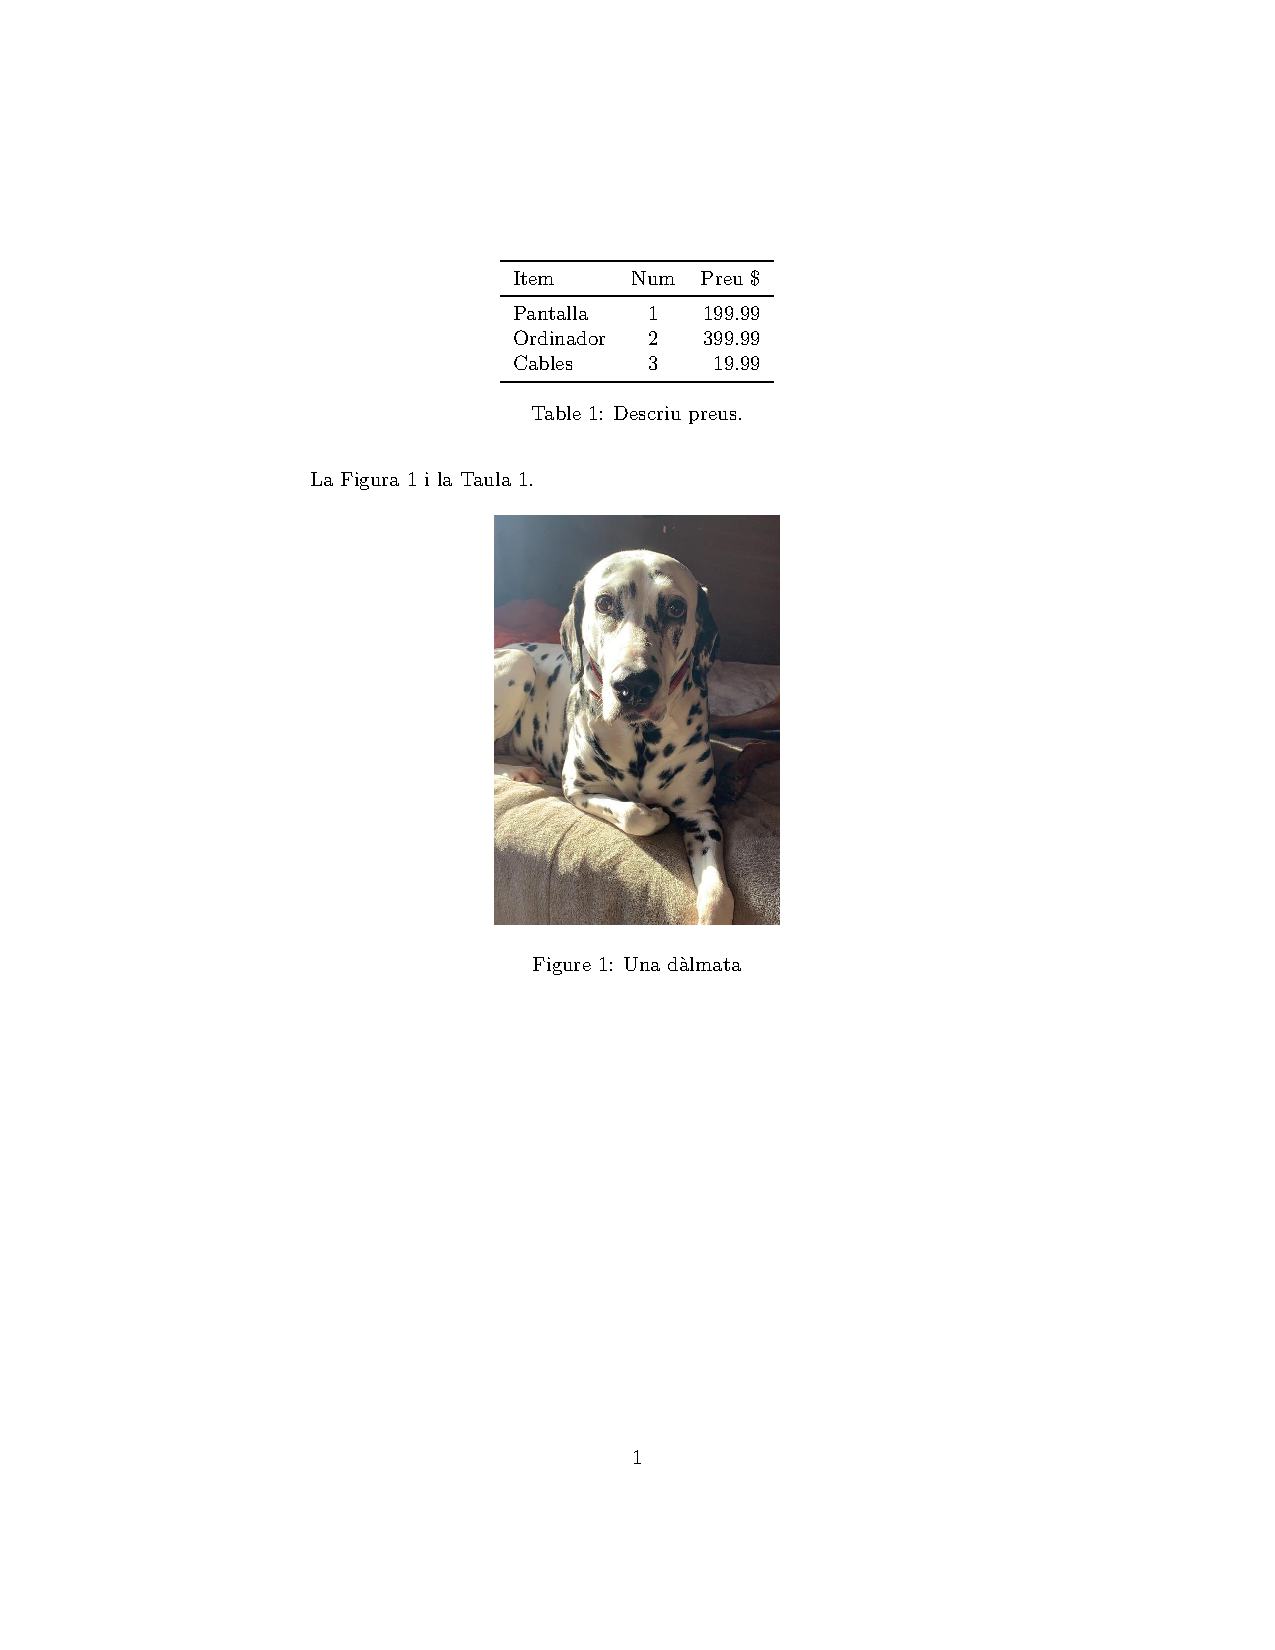
\includegraphics[width=\textwidth,clip,trim=2in 3in 3in 1in]{media-graphics-tables.pdf}
\end{minipage}
\end{frame}

%%%%%%%%%%%%%%%%%%%%%%%%%%%%%%%%%%%%%%%%%%%%%%%%%%%%%%%%%%%%%%%%%%%%%%%%%%%%%%%
%%%%%%%%%%%%%%%%%%%%%%%%%%%%%%%%%%%%%%%%%%%%%%%%%%%%%%%%%%%%%%%%%%%%%%%%%%%%%%%
%%%%%%%%%%%%%%%%%%%%%%%%%%%%%%%%%%%%%%%%%%%%%%%%%%%%%%%%%%%%%%%%%%%%%%%%%%%%%%%
\begin{frame}[fragile]{Repassem: Matemàtiques}
\begin{itemize}
\item Els símbols de dòlar \keystrokebftt{\$} marquen matemàtiques al text.
\begin{exampletwouptiny}
% meh:
Siguin a i b nombres enters 
positius, i sigui c > a - b + 1

% millor:
Siguin $a$ i $b$ nombres enters 
positius, i sigui $c > a - b + 1$.
\end{exampletwouptiny}
\item Utilitza sempre els símbols de dòlar amb parelles: un per començar les matemàtiques, i un per acabar-les.
\end{itemize}
\end{frame}

%%%%%%%%%%%%%%%%%%%%%%%%%%%%%%%%%%%%%%%%%%%%%%%%%%%%%%%%%%%%%%%%%%%%%%%%%%%%%%%
%%%%%%%%%%%%%%%%%%%%%%%%%%%%%%%%%%%%%%%%%%%%%%%%%%%%%%%%%%%%%%%%%%%%%%%%%%%%%%%
%%%%%%%%%%%%%%%%%%%%%%%%%%%%%%%%%%%%%%%%%%%%%%%%%%%%%%%%%%%%%%%%%%%%%%%%%%%%%%%
\begin{frame}[fragile]{Taules: més opcions}
Hi ha moltes opcions diferents per fer taules.
\begin{itemize}
\item Es poden fusionar columnes amb \cmdbs{multicolumn} i files amb \cmdbs{multirow} (cal el paquet \bftt{multirow}).
\item Línies horitzontals més curtes amb \cmdbs{cline} o \cmdbs{cmidrule} de \bftt{booktabs}.
\end{itemize}

\begin{exampletwouptiny}
\begin{tabular}{lrr}
\toprule
Item &
\multicolumn{2}{c}{MultiColumna} \\
\cline{2-3}
Pantalla                   & 1 & 2.99\\
\cmidrule{1-2}
\multirow{2}{*}{MultiFila} & 2 & 3.99\\
                           & 3 & 1.99\\
\bottomrule
\end{tabular}
\end{exampletwouptiny}
\end{frame}

\end{document}

%%%%%%%%%%%%%%%%%%%%%%%%%%%%%%%%%%%%%%%%%%%%%%%%%%%%%%%%%%%%%%%%%%%%%%%%%%%%%%%
%%%%%%%%%%%%%%%%%%%%%%%%%%%%%%%%%%%%%%%%%%%%%%%%%%%%%%%%%%%%%%%%%%%%%%%%%%%%%%%
%%%%%%%%%%%%%%%%%%%%%%%%%%%%%%%%%%%%%%%%%%%%%%%%%%%%%%%%%%%%%%%%%%%%%%%%%%%%%%%
\begin{frame}[fragile]{Repassem: Estructura Documents}
\begin{itemize}{\small
\item Comença amb \cmdbs{documentclass} --- quin tipus de document.
\item Metadades (\cmdbs{title} i \cmdbs{author}) i paquets en el preàmbul. 
\item Contingut entre \cmdbegin{document} i \cmdend{document}.
\item L'ordre \cmdbs{maketitle} crea el títol; \cmdbs{section} crea seccions numerades.
}\end{itemize}
\begin{minipage}{0.55\linewidth}
\inputminted[fontsize=\scriptsize,frame=single,resetmargins]{latex}%
  {recap-structure.tex}
\end{minipage}
\begin{minipage}{0.35\linewidth}
% trim: l b r t

\includegraphics[width=\textwidth,clip,trim=1.5in 7in 3in 2in]{recap-structure.pdf}
\end{minipage}
\end{frame}

%%%%%%%%%%%%%%%%%%%%%%%%%%%%%%%%%%%%%%%%%%%%%%%%%%%%%%%%%%%%%%%%%%%%%%%%%%%%%%%
%%%%%%%%%%%%%%%%%%%%%%%%%%%%%%%%%%%%%%%%%%%%%%%%%%%%%%%%%%%%%%%%%%%%%%%%%%%%%%%
%%%%%%%%%%%%%%%%%%%%%%%%%%%%%%%%%%%%%%%%%%%%%%%%%%%%%%%%%%%%%%%%%%%%%%%%%%%%%%%
\begin{frame}[fragile]{Repassem: Exercici}

\begin{enumerate}
\item Aquí teniu un text per un article curt:\footnote{Basat en \url{http://www.cgd.ucar.edu/cms/agu/scientific_talk.html}}
\begin{center}
\fbox{\href{\wlnewdoc{recap-exercise.tex}}{%
Cliqueu per obrir l'exercici a \wllogo{}}}
\end{center}
\vskip 2ex
\item Afegiu ordre de \LaTeX{} perquè tingui el mateix aspecte que el següent:
\begin{center}
\fbox{\href{\fileuri/recap-exercise-solution.pdf} amb una barra inversa (\cmdbs{\%}).
\end{itemize}
\end{block}
\end{frame}
